\documentclass[12pt, leqno]{article} %% use to set typesize

\usepackage{amsmath}
\usepackage{amssymb}
\usepackage{enumerate}
\usepackage{tikz}
\usetikzlibrary{arrows,positioning, calc}
\tikzstyle{vertex}=[draw,circle,minimum size=20pt,inner sep=0pt]

%\usepackage{minted}

%\usepackage{fontspec}
%\setmonofont[
%  Extension      = .ttf ,
%  Ligatures      = {NoCommon, NoRequired, NoContextual, NoHistoric, NoDiscretionary},
%  UprightFont    = * ,
%  ItalicFont     = *-Oblique ,
%  BoldFont       = *-Bold ,
%  BoldItalicFont = *-BoldOblique
%]{DejaVuSansMono}

\usepackage{fancyhdr}
\pagestyle{fancy}

\makeatletter
\renewcommand{\maketitle}{\bgroup\setlength{\parindent}{0pt}
\begin{flushleft}
  {\Large\vspace*{-0.5in}\textsc{\@title}}\newline
  CS 2112 Fall 2016
  \rule{\textwidth}{1pt}
\end{flushleft}\egroup
}
\makeatother


\renewcommand{\headrulewidth}{0pt}
\setlength{\headheight}{0.5in}
\lhead{Recitation 7}
\rhead{CS 2112 Fall 2016}
\title{ASTs, Regex, Parsing, and Pretty Printing}
\begin{document}
\thispagestyle{empty}
\vspace*{-0.5in}
\maketitle
%
%%
%%%
%%%%
%%%%% section algebraic_expressions
%%%%%
%%%%%
%%%%%
%%%%%
\section{Algebraic Expressions}
\label{sec:algebraic_expressions}
To start, consider integer arithmetic.  Suppose we have the following
\begin{enumerate}
  \item The \emph{alphabet} we will use is the digits $\{0,~1,~2,~3,~4,~5,~6,~7,~8,~9\}$.
  \item We will allow the unary operator (one argument) $-$ for negation.
  \item We will allow the binary operators:
  \begin{center}
    \begin{tabular}{c|l}
      $+$    & addition       \\
      $-$    & subtraction    \\
      $\ast$ & multiplication \\
      $/$    & division       \\
    \end{tabular}
  \end{center}
\end{enumerate}
For ease and clarity of presentation, when we represent expressions as Abstract Syntax Trees (AST),
we will only allow for two children for a given operation.  In this is the maximum allowed,
as we only have binary operators.  However, we will see ASTs later that will be more flexible.\\

\noindent Consider the following AST for integer algebra

\begin{center}
  \begin{tikzpicture}[thick,level/.style={sibling distance=60mm/#1}]
    \node [vertex] {$\ast$}
      child {
        node [vertex] {$+$}
        child {
          node [vertex] {$3$}
        }
        child {
          node [vertex] {$5$}
        }
      }
      child {
        node [vertex] {$4$}
      };
  \end{tikzpicture}
\end{center}
We parse it left to right, and bottom up, so it represents the expression
\[
  (3 + 5) * 4
\]
equally important, it is very much \textbf{not}
\[
  3 + 5 * 4
\]
\newpage
\noindent Another example:
\begin{center}
  \begin{tikzpicture}[thick,level/.style={sibling distance=60mm/#1}]
    \node [vertex] {$-$}
      child {
        node [vertex] {$\ast$}
        child {
          node [vertex] {$+$}
          child {
            node [vertex] {$3$}
          }
          child {
            node [vertex] {$5$}
          }
        }
        child {
          node [vertex] {$/$}
          child {
            node [vertex] {$32$}
          }
          child {
            node [vertex] {$2$}
          }
        }
      };
  \end{tikzpicture}
\end{center}
This example represents the expression
\[
  -(~(3 + 5)~\ast~(32 / 2)~)
\]
Before continuing with more examples, lets revisit regular expressions.
%%%%%
%%%%%
%%%%%
%%%%%
%%%%% section algebraic_expressions
%%%%
%%%
%%
%

%
%%
%%%
%%%%
%%%%% section regular_expression_review
%%%%%
%%%%%
%%%%%
%%%%%
\section{Regular Expression Review}
\label{sec:regular_expression_review}
\subsection{The ``alphabet'' of regular expressions}
The alphabet of a regular expression is denoted by $\Sigma$.  This \emph{set} is what
defines what are ``valid'' components of the regular expression.  For example,
\begin{enumerate}
  \item $\Sigma = \{0,~1\}$

  This is the alphabet of all \emph{binary} strings, encoded as \emph{0}'s and \emph{1}'s.

  \item $\Sigma = \{a,~b,~c\}$

  This is the alphabet of all strings that contain either
  \begin{enumerate}[i)]
    \item all \emph{a}'s
    \item all \emph{b}'s
    \item all \emph{c}'s
    \item all \emph{a}'s and \emph{b}'s
    \item all \emph{a}'s and \emph{c}'s
    \item all \emph{b}'s and \emph{c}'s
    \item all \emph{a}'s and \emph{b}'s and \emph{c}'s
  \end{enumerate}
As you can see, the ability to define the alphabet of a regular expression using set
notation is exceptionally convenient.
\end{enumerate}

\subsection{The \emph{Kleene Star} ($\ast$) is a post-fix operator}

This operator represents \emph{0 or more} occurrences of whatever it operates on.  For example,
\begin{enumerate}
  \item $d^\ast~\longrightarrow~\{\varepsilon,~d,~dd,~ddd,~\cdots\}$
  \item $(01)^\ast~\longrightarrow~\{\varepsilon,~01,~0101,~010101,~\cdots\}$
  \item If $\Sigma = \{a,~b\}$, then $\Sigma^\ast = \{\varepsilon,~a,~b,~ab,~ba,~aab,~aba,~baa,~\cdots\}$
\end{enumerate}
where $\varepsilon$ is the \emph{empty} string.  Later, we will use $\varnothing$ to represent the empty set.

\subsection{A plus sign $(+)$ represents a \emph{union}}

Recalling that regular expressions are \emph{sets}, we use the notation
\[
  A + B \longrightarrow A \cup B
\]
For example,

\begin{enumerate}
  \item $\{a,~b\} + \{c,~d\} = \{a,~b,~c,~d\}$
  \item $\{a,~b,~c\} + \{b,~c,~d\} = \{a,~b,~c,~d\}$
\end{enumerate}
When we use $+$, it is a binary operator (it requires two arguments).  Additionally, note that the unions
produced do not have duplicated elements -- in the second example, we do not have duplicate $b$ or $c$.

\subsection{A dot product $(\cdot)$ represents a \emph{concatenation}}

We use the notation
\[
  A \cdot B \longrightarrow \{xy~|~x\in A,~y \in B\}
\]
For example,

\begin{enumerate}
  \item $\{a,~b\}\cdot\{c,~d\} = \{ac,~ad,~bc,~bd\}$
  \item $\{a,~b,~c\}\cdot\{b,~c,~d\} = \{ab,~ac,~ad,~bb,~bc,~bd,~cb,~cc,~cd\}$
\end{enumerate}

%%%%%
%%%%%
%%%%%
%%%%%
%%%%% section regular_expression_review
%%%%
%%%
%%
%
%
%%
%%%
%%%%
%%%%% section ast_s_and_regular_expressions
%%%%%
%%%%%
%%%%%
%%%%%
\section{AST's and regular expressions}
\label{sec:ast_s_and_regular_expressions}
Consider the AST
\begin{center}
  \begin{tikzpicture}[thick,level/.style={sibling distance=100mm/#1}]
    \node [vertex] {$\ast$}
      child {
        node [vertex] {$+$}
        child {
          node [vertex] {$a$}
        }
        child {
          node [vertex] {$\cdot$}
          child {
            node [vertex] {$\cdot$}
            child {
              node [vertex] {$b$}
            }
            child {
              node [vertex] {$\ast$}
              child {
                node [vertex] {$\cdot$}
                child {
                  node [vertex] {$\cdot$}
                  child {
                    node [vertex] {$a$}
                  }
                  child {
                    node [vertex] {$\ast$}
                    child {
                      node [vertex] {$b$}
                    }
                  }
                }
                child {
                  node [vertex] {$a$}
                }
              }
            }
          }
          child {
            node [vertex] {$b$}
          }
        }
      };
  \end{tikzpicture}
\end{center}
This describes the regular expression
\[
  (~a~+~b~(~ab^\ast a~)^\ast~b~)^\ast
\]
which, when written as parsed from above with parentheses to group (parentheses colored to help hit be a little more understandable):
\[
  \textcolor{blue}{(}a~+~(\textcolor{red}{(}b~\cdot~(\textcolor{blue}{(}a~\cdot~b^\ast\textcolor{blue}{)}~\cdot~a)^\ast\textcolor{red}{)}~\cdot~b)\textcolor{blue}{)}^\ast
\]
%%%%%
%%%%%
%%%%%
%%%%%
%%%%% section ast_s_and_regular_expressions
%%%%
%%%
%%
%
%
%%
%%%
%%%%
%%%%% section alternate_interpretation_of_regular_expressions
%%%%%
%%%%%
%%%%%
%%%%%
\section{Alternate interpretation}
\label{sec:alternate_interpretation_of_regular_expressions}
As it turns out, we can use (deterministic) finite state machines to represent the regular expression presented in Section \ref{sec:ast_s_and_regular_expressions}.  The state machine would be as follows:

\begin{center}
  \begin{tikzpicture}[scale=0.2]
    \tikzstyle{every node}+=[inner sep=0pt]
    \draw [black] (16.5,-26.2) circle (3);
    \draw (16.5,-26.2) node {Start};
    \draw [black] (16.5,-26.2) circle (2.4);
    \draw [black] (34.6,-26.2) circle (3);
    \draw (34.6,-26.2) node {$S_0$};
    \draw [black] (53.7,-26.2) circle (3);
    \draw (53.7,-26.2) node {$S_1$};
    \draw [black] (13.82,-27.523) arc (324:36:2.25);
    \draw (9.25,-26.2) node [left] {$a$};
    \fill [black] (13.82,-24.88) -- (13.47,-24) -- (12.88,-24.81);
    \draw [black] (17.414,-23.357) arc (152.77578:27.22422:9.149);
    \fill [black] (33.69,-23.36) -- (33.76,-22.42) -- (32.87,-22.87);
    \draw (25.55,-17.89) node [above] {$b$};
    \draw [black] (35.4,-23.321) arc (155.52508:24.47492:9.614);
    \fill [black] (52.9,-23.32) -- (53.02,-22.39) -- (52.11,-22.8);
    \draw (44.15,-17.19) node [above] {$a$};
    \draw [black] (56.147,-24.485) arc (152.74616:-135.25384:2.25);
    \draw (61.07,-24.98) node [right] {$b$};
    \fill [black] (56.55,-27.1) -- (57.03,-27.91) -- (57.49,-27.02);
    \draw [black] (52.899,-29.078) arc (-24.49465:-155.50535:9.614);
    \fill [black] (35.4,-29.08) -- (35.28,-30.01) -- (36.19,-29.6);
    \draw (44.15,-35.21) node [below] {$a$};
    \draw [black] (34.071,-29.139) arc (-19.6923:-160.3077:9.051);
    \fill [black] (17.03,-29.14) -- (16.83,-30.06) -- (17.77,-29.72);
    \draw (25.55,-35.64) node [below] {$b$};
  \end{tikzpicture}
\end{center}
So in this example, the start state and the accept state (double circle) are the same thing.  Convince yourself that the regular expression
\[
  (~a~+~b~(~ab^\ast a~)^\ast~b~)^\ast
\]
is correctly represented by the finite state machine above by following the arrows.  For example, if we saw the string ``ba'' then we would go from the ``Start'' state, to state ``$S_0$'', to state ``$S_1$''.  This string would not be accepted by the finite state machine, which is good because it is not described by the regular expression.\\

\noindent On the other hand, consider the string ``$abbbabbbbbbbab$''.  Follow the edges to see.  The input will put you at the following states:
\begin{center}
  \begin{tabular}{|c|c|c|c|c|c|c|c|c|c|c|c|c|c|c|c|c|c|}
    \hline
    $a$ & $b$ & $b$ & $b$ & $a$ & $b$ & $b$ & $b$ & $b$ & $b$ & $b$ & $b$ & $a$ & $b$ \\ \hline
    Start & $S_0$ & Start & $S_0$ & $S_1$ & $S_1$ & $S_1$ & $S_1$ & $S_1$ & $S_1$ & $S_1$ & $S_1$ & $S_0$ & Start\\ \hline
  \end{tabular}
\end{center}
So we can see that there is a direct relationship between the Kleene Star and self-loops in a state machine.  Abstract Syntax Trees and Finite State Machines are both excellent conceptual models for understanding regular expressions, but they are not the only ones.  In fact, they are just barely the tip of the iceberg!
%%%%%
%%%%%
%%%%%
%%%%%
%%%%% section alternate_interpretation_of_regular_expressions
%%%%
%%%
%%
%
%
%%
%%%
%%%%
%%%%% section pretty_printing
%%%%%
%%%%%
%%%%%
%%%%%
\section{Pretty Printing}
\label{sec:pretty_printing}
When it comes to pretty printing ASTs, recursion should feel the most natural.  Accompanying this PDF is a full version of the snippet below, in \texttt{PrettyPrint.java}.\\

\noindent An excerpt from the program is sufficient for explaining the idea:
%\begin{minted}[fontsize=\footnotesize]{java}
\begin{small}
\begin{verbatim}
/* Class Node has
 * 
 *     Node[] children = new Node[2];
 *
 * where the following invariant is maintained:
 *
 * - Index 0 and 1 are null:                terminal node
 * - Index 0 has value and index 1 is null: unary operator
 * - Index 0 is null and index 1 has value: post-fix operator
 * - Index 0 and index 1 both have values:  binary operator
 *
 * Clearly this tactic does not scale well, but illustrates the concept.
 */
public static void prettyPrint(Node n) {
    // terminal nodes just get printed
    if(n.isTerminal()) {
        System.out.print(n);
    }
    // print the unary op followed by its only child
    else if(n.isUnaryOp()) {
        System.out.print(n);
        prettyPrint(n.children[0]);
    }
    // post-fix operators get printed after their only child
    else if(n.isPostFixOp()) {
        prettyPrint(n.children[1]);
        System.out.print(n);
    }
    // binary operators, print the left child first, the op, then right
    else if(n.isBinaryOp()) {
        System.out.print("(");
        prettyPrint(n.children[0]);
        System.out.print(" " + n + " ");
        prettyPrint(n.children[1]);
        System.out.print(")");
    }
}
\end{verbatim}
\end{small}
%\end{minted}
%%%%%
%%%%%
%%%%%
%%%%%
%%%%% section pretty_printing
%%%%
%%%
%%
%
\end{document}
